\documentclass[11pt]{article}
\usepackage[margin=1in, top=1in]{geometry}
\usepackage[all]{nowidow}
\usepackage[hyperfigures=true, hidelinks, pdfhighlight=/N]{hyperref}
\usepackage[separate-uncertainty=true, group-digits=false]{siunitx}
\usepackage{graphicx,amsmath,physics,tabto,float,amssymb,pgfplots,verbatim,tcolorbox}
\usepackage{listings,xcolor,subcaption,caption,import,wrapfig,minted}
\usepackage[sorting=none]{biblatex}
\usepackage[version=4]{mhchem}
\usepackage[noabbrev]{cleveref}
\usepackage[british]{babel}
\newcommand{\creflastconjunction}{, and\nobreakspace}
\newcommand{\mb}[1]{\mathbf{#1}}
\numberwithin{equation}{section}
\numberwithin{figure}{section}
\numberwithin{table}{section}
\captionsetup{font=small, belowskip=0pt}
\pgfplotsset{compat=1.17}
\addbibresource{bibliography.bib}
\usemintedstyle{vs}
\definecolor{LightGray}{HTML}{eaeaea}
\setminted{framesep=2mm,bgcolor=LightGray,fontsize=\footnotesize,linenos,breaklines}
\addbibresource{bibliography.bib}

\begin{document}

\begin{center}
    {\huge Investigating the gamma-ray spectra of radiation sources 152Eu and AmBe}\\
    \vspace{0.2in}
    \textbf{KDSMIL001 | October 2022}
\end{center}


\section{Introduction}\label{sec:Introduction}
There are many sources of photon radiation naturally present in the world. Gamma-rays (roughly between \SI{0.001}{\mega\electronvolt} and \SI{10}{\mega\electronvolt}) are the highest energy and thus most dangerous form of photon radiation. For this reason, understanding where gamma-rays come from and how they interact with matter is of great importance. 

This report will discuss the origins of gamma-rays and how they are detected, and then analyse the gamma-ray spectra from two radiation sources---\ce{^{152}Eu} and AmBe---with reference to the expectation according to theory as well as previous experiment. The NaI scintillation detector and multi-channel analyser that were used needed to be calibrated to output energy so the standard \ce{^{22}Na}, \ce{^{60}Co}, and \ce{^{137}Cs} calibration sources were used. The energy resolution of the NaI scintillation detector was also determined using the calibration sources for discussion about the sources of interest.

\section{Theory}\label{sec:Theory}

\subsection{Gamma-rays}\label{sec:GammaTheory}
One of the main sources of gamma-rays is from the de-excitation of atomic nuclei. Similar to how electrons surrounding the nucleus can be excited and then emit a photon (usually an X-ray) when they de-excite, the nuclei of atoms can be excited and when they drop down to a lower energy, they emit a photon. Due to the greater mass of nuclei compared to electrons, their possible states have a much larger energy gap and thus the energy of the emitted photons is far greater. These energy levels are also very well defined, so for a given nucleus, we expect to see gamma-rays at specific, given energies. 

Unlike electrons, nuclei don't often get excited simply by an incoming photon simply because the likelihood of a gamma-ray of the right energy being in the right place is so low. For this reason, the vast majority of gamma-rays that we see come either from nuclear decays or nuclear reactions. When a radionuclide decays, it has a chance to decay to a daughter nucleus that is not in its ground state. The daughter nucleus can then de-excite by emission of a gamma-ray. The half-life of this excited state is usually on the order of picoseconds while the common radionuclides that we see in the lab have half-lives on the order of at least a few months, if not years. We can then quite confidently correlate gamma-ray emission (and thus detection) with a decay. In a similar way when nuclei gain nucleons through some nuclear process\footnote[1]{Extra marks for alliteration?}, they can also become excited and thus decay by emission of a gamma-ray. 

\subsection{Detector theory}\label{sec:DetectorTheory}
The detector used in this experiment is a NaI (Sodium Iodide) crystal scintillation detector. These detectors are designed to detect photons and work by the following principles. When a photon passes through the detector material it has 3 ways of depositing its energy onto the detector. It can either be completely absorbed by an atom through photoelectric absorption (resulting in an energetic photoelectron that gets ejected from the atom), Compton scatter off an electron in the material (and send the electron flying), or pair produce an electron-positron pair. These processes all result in an electron (or positron) travelling freely through the detector material that excites other electrons in the crystal lattice. These electrons de-excite by emission of a visible light photon that is directed to the cathode of a high voltage photomultiplier tube, which turns the signal into a voltage pulse that is (hopefully) proportional to the energy of the initial photon.

The 3 processes which result in the free electrons have different relative cross-sections at different photon energies. The photoelectric effect is most dominant at low energies, dropping off as energy increases; pair production can only start at an energy of \SI{1.022}{\mega\electronvolt}, as it needs to produce an electron and positron, and only gets more dominant from that point; and Compton scattering takes over between the two. This is relevant as the 3 processes have distinct signatures when looking at gamma-ray spectra. The photoelectric effect is effectively lossless, with all the photon's energy being transferred to the electron and thus onto the detector. Compton scattering, however, is limited by the kinematics of the situation meaning it can only ever deposit a fraction of the photon energy in one interaction. This leads to a so-called Compton continuum that begins at very low energies and stops at the Compton edge, the energy of which is related to the original photon energy by 
\begin{equation}
    E_\mathrm{Compton}=\frac{2E_\gamma^2}{m_e c^2 + 2E_\gamma}.
\end{equation}
Pair production produces an electron-positron pair. The electron is very likely to behave well and deposit all its energy, but the positron has a high likelihood of annihilating with electrons in the crystal and producing back-to-back \SI{511}{\kilo\electronvolt} photons. These photons can be absorbed again and all is good, or one or both of them could escape the detector with all their energy. Thus, for photons greater than \SI{1022}{\kilo\electronvolt} we expect to see two ``escape peaks'' at \SI{511}{\kilo\electronvolt} and \SI{1022}{\kilo\electronvolt} below the original energy. 

\section{Apparatus}\label{sec:Apparatus}
The apparatus was configured as in \cref{fig:Apparatus}. The detector is an NaI scintillator detector and photomultiplier tube. The preamplifier is an ORTEC model 113. The amplifier is an ORTEC model 572. The MCA is a SPECTECH UCS-30. The oscilloscope was used simply for monitoring. The HV was set to \SI{700}{\volt}.

\begin{figure}[h]
    \begin{center}
        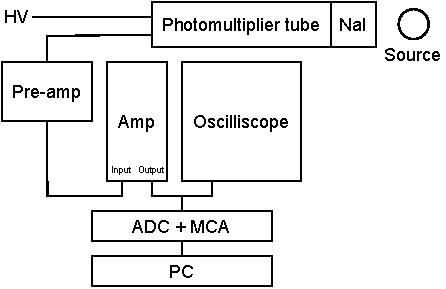
\includegraphics[width=.4\textwidth]{Plots/apparatus.pdf}
        \caption{Schematic of the set-up used in the experiment.}
        \label{fig:Apparatus}
    \end{center}
\end{figure}

\section{Calibration \& Energy Resolution}\label{sec:CalibrationResolution}
The radioactive sources used for calibration were \ce{^{22}Na}, \ce{^{60}Co}, and \ce{^{137}Cs}. A gamma spectrum was captured for a live time of \SI{1200}{\second} for each source. A background reading of \SI{1200}{\second} was also recorded. Two energy ranges were needed so this was done twice, reducing the gain on the amplifier for the second run in order to reach a higher energy in the highest bin of the MCA. 

For both configurations, the channel number for the centroid value of each photopeak was determined by fitting a gaussian. A scatter plot was made relating channel number to expected photopeak energy (sourced from NuDat3~\cite{nudat}) and a straight line fitted. Standard deviation on the fitted gaussians was used as uncertainty on the channel number. The scatter plots for each calibration are shown in \cref{fig:calibration}.

\begin{figure}[h]%
    \centering
    \begin{subfigure}[t]{.49\linewidth}
        \centering
        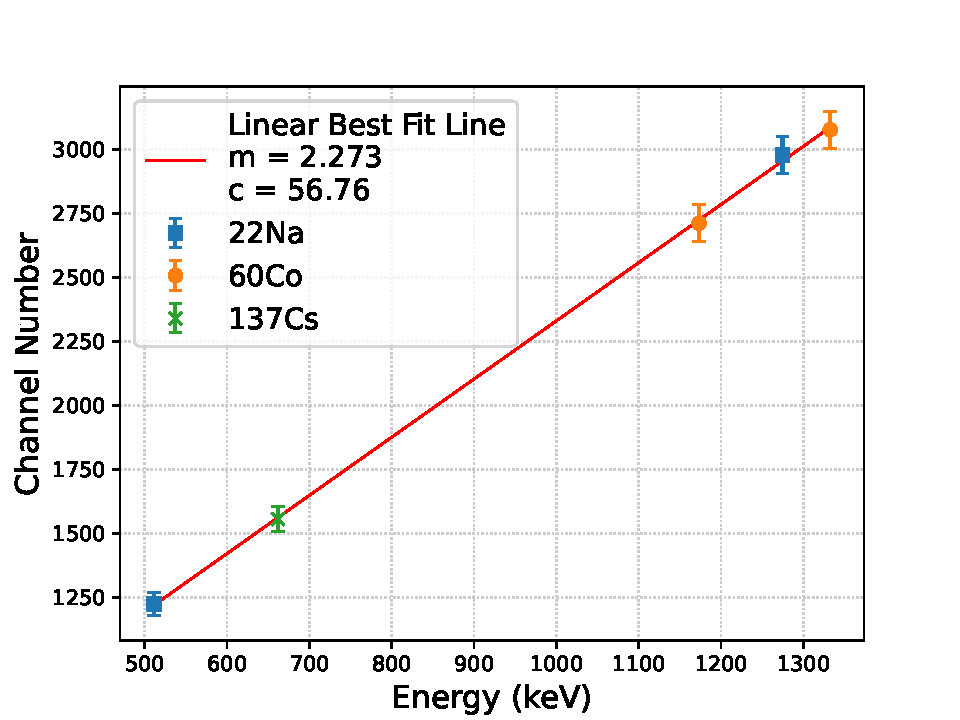
\includegraphics[width=\linewidth]{Plots/low_calibration.pdf}
        \caption{Scatter plot and fitted line for the low energy calibration. The largest energy resolvable with this calibration was \SI{1776}{\kilo\electronvolt}.}
        \label{fig:low_calibration}
    \end{subfigure}
    \hfill
    \begin{subfigure}[t]{.49\linewidth}
        \centering
        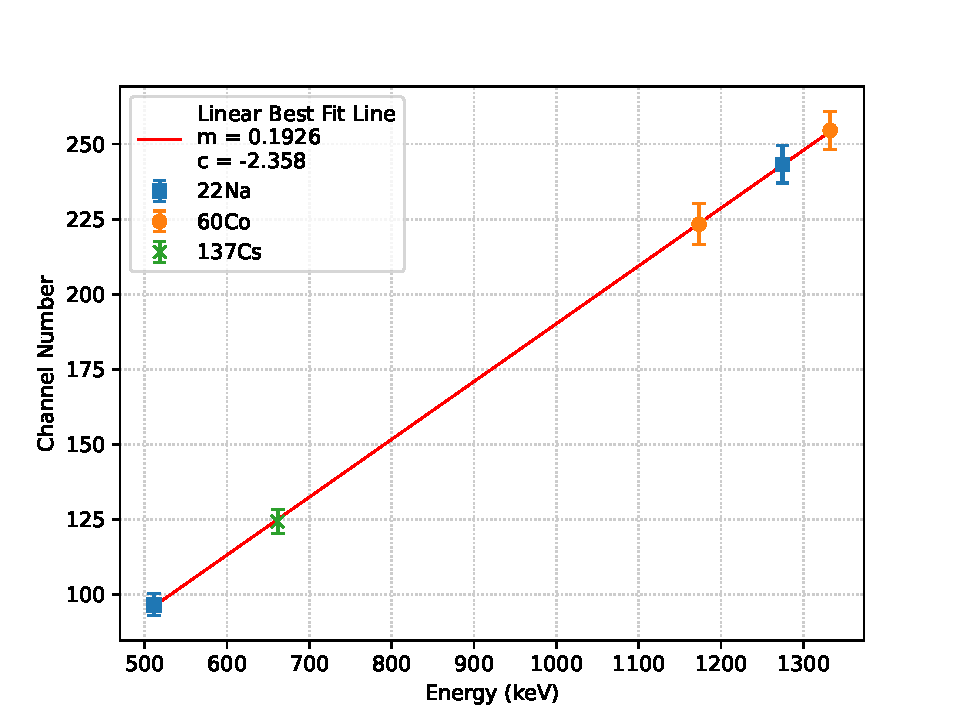
\includegraphics[width=\linewidth]{Plots/high_calibration.pdf}
        \caption{Scatter plot and fitted line for the high energy calibration. The largest energy resolvable with this calibration was \SI{5330}{\kilo\electronvolt}.}
        \label{fig:high_calibration}
    \end{subfigure}
\caption{}
\label{fig:calibration}
\end{figure}

To find the energy resolution, the primary photopeaks of the calibration sources were used. Using the standard deviation found earlier, the FWHM was found with $FWHM=2\sqrt{2\ln(2)}\sigma$ and the energy resolution found from \cite[Fig. 4.5]{Knoll}:

\begin{equation}
    R=\frac{FWHM}{H_0}
    \label{eqn:EnergyResolution}
\end{equation}
where $H_0$ is the mean of the gaussian. Taking the mean of the 5 values, a resolution of 6.855\% was found. This means that for a photon of a given energy $E$, there will be a range with width $6.855\%\times E$ around that energy for which a photon of a different energy to the original will not be resolvable as being a different energy. 

\section{\ce{^{152}Eu}}\label{sec:Eu}

\subsection{\ce{^{152}Eu} Theory}
\ce{^{152}Eu} is a radioisotope of \ce{_{63}Eu}. In its ground state it decays by $\beta^-$ emission with an intensity of 27.9\% and electron capture ($\varepsilon$) with an intensity of 72.1\%~\cite{nudat}. Both decays result in gamma-rays but they result in completely different spectra. The expected spectrum, however, must be a combination of the two. 

\subsection{\ce{^{152}Eu} Gamma Spectrum}
\Cref{fig:Eu_Spectrum} shows the gamma-ray spectrum for \ce{^{152}Eu}. This data was taken with a live time of \SI{1200}{\second}, then all counts were divided by 1200 to normalise in time. A background reading of the same live time was taken, normalised, and subtracted from the initial before any analysis was done. The AmBe source was a large contributor of background radiation.

Labelled in \cref{fig:Eu_Spectrum} are the energies of the expected gamma-rays with the highest intensities according to \cite{nudat}. It is evident from the plot that at high energies the expected energies are lower than the energies output by the detector after calibration and at low energies the expected energies are higher than the detector output. This seems to imply that the slope of the line determined in calibration, for the low energy regime at least, must be incorrect. 

\begin{figure}[h]
    \begin{center}
        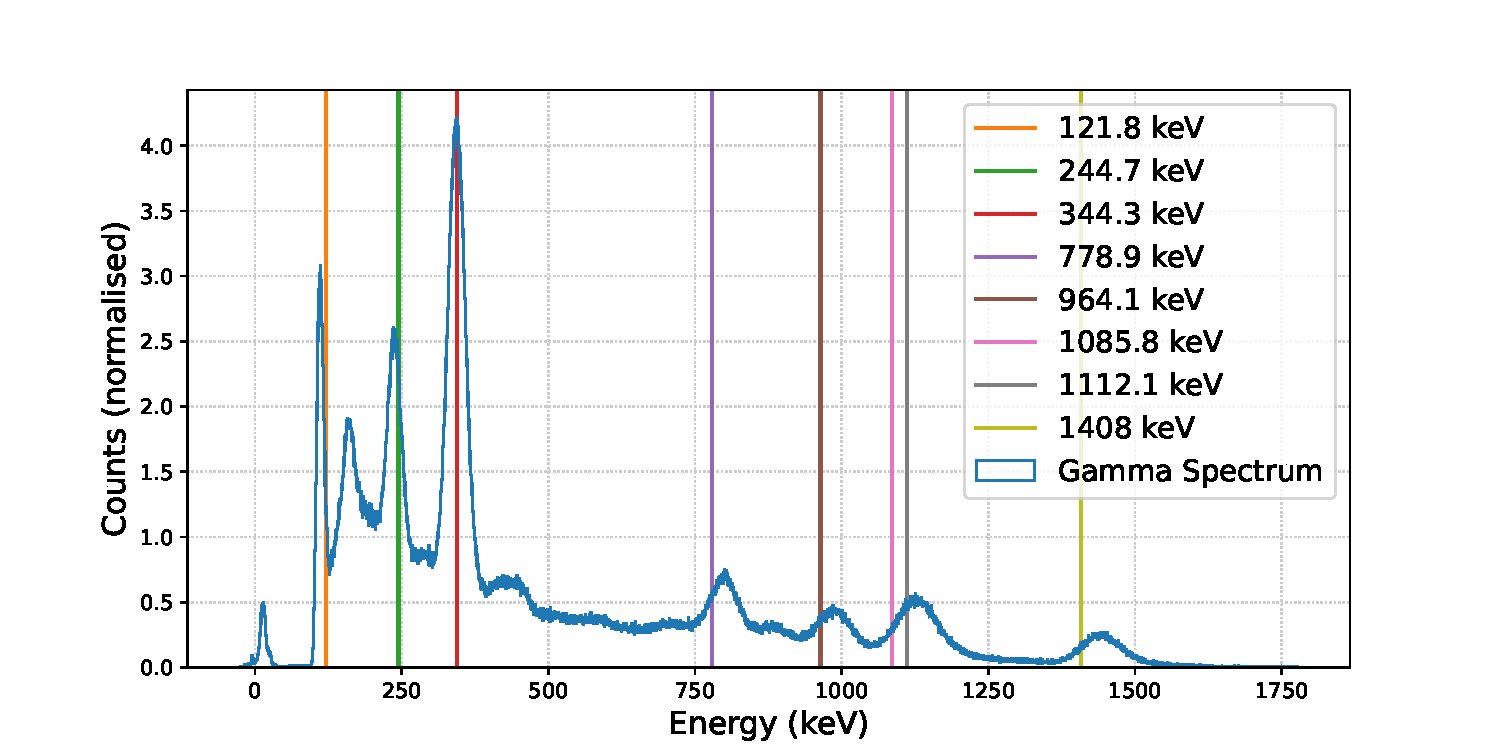
\includegraphics[width=.8\textwidth]{Plots/eu.pdf}
        \caption{Gamma-ray spectrum for the \ce{^{152}Eu} source after normalising with respect to time and subtracting background. The most prominent expected gamma-ray emission energies are labelled. Note how for high energies the expected energy is lower than detected and for low energies the opposite is true.}
        \label{fig:Eu_Spectrum}
    \end{center}
\end{figure}

Many of the gamma-rays in the expected \ce{^{152}Eu} spectrum are close to each other in energy, but there are only a few that have a large enough intensity that they are visible in the spectrum. The gamma-rays of energy \SI{1085.8}{\kilo\electronvolt} and \SI{1112.1}{\kilo\electronvolt} are two such emissions. Considering the energy resolution calculated in \cref{sec:CalibrationResolution}, both photons lie within the other's resolution range so they are not resolvable as two different peaks. This is made worse by the fact that they have similar intensities (10.11\% and 13.67\% respectively), leading to what looks like just one photopeak in \cref{fig:Eu_Spectrum}.

\section{AmBe}\label{sec:AmBe}

\subsection{AmBe Theory}\label{sec:AmBeTheory}
The Americium-Beryllium (AmBe) source is primarily a neutron source. $\alpha$ particles are emitted by the \ce{^{241}Am} source leading to the process

\begin{equation}
    \alpha + \ce{^{9}Be} \rightarrow \ce{^{13}C^*} \rightarrow \ce{^{12}C^*}+n \rightarrow \ce{^{12}C}+n+\gamma_{\SI{4439.82}{\kilo\electronvolt}}.
    \label{eqn:AmBeProcess}
\end{equation}
The photon is mono-energetic but the neutrons are emitted with a wide range of energies including thermal neutrons. Thermal neutrons are very likely to be captured by material surrounding the AmBe source. The source used in this lab was surrounded by high density plastic, which is primarily made up of hydrogen and carbon, so it is expected to have excited deuterium (D or \ce{^{2}H}) and \ce{^{13}C} produced. 

The expected energy of the photon released as deuterium de-excited can be found by looking at the binding energy. The mass of deuterium is \SI{2.0135533893}{u}~\cite{deuterium} and the mass of its constituent parts is \SI{2.01594147}{u}, from the neutron and proton mass. The mass excess is then \SI{2.3880807e-3}{u} leaving a binding energy of \SI{2224.497}{\kilo\electronvolt}. So, when the hydrogen captures a neutron and becomes deuterium, it will end up in an excited state with an energy of \SI{2224.497}{\kilo\electronvolt}. Thus a gamma-ray of that energy should be expected in the AmBe spectrum. 

The deuterium gamma-ray and the \SI{4439.82}{\kilo\electronvolt} gamma-ray from carbon are both above the pair production threshold, so single- and double-escape peaks should be expected. 

\subsection{AmBe Gamma Spectrum}
\Cref{fig:AmBe_Spectrum} shows the gamma-ray spectrum for the AmBe source. Data was taken with a live time of about \SI{13000}{\second} and the counts were divided by that to normalise in time. No background reading was taken as the detector and AmBe source could both not be moved. On the spectrum, the gamma-rays mentioned in \cref{sec:AmBeTheory} are labelled. The escape peaks of the deuterium peak are not labelled as they are saturated by the bremsstrahlung and Compton continua and thus not visible. An unknown gamma-ray is present that doesn't seem to align with any expectation. 

\begin{figure}[h]
    \begin{center}
        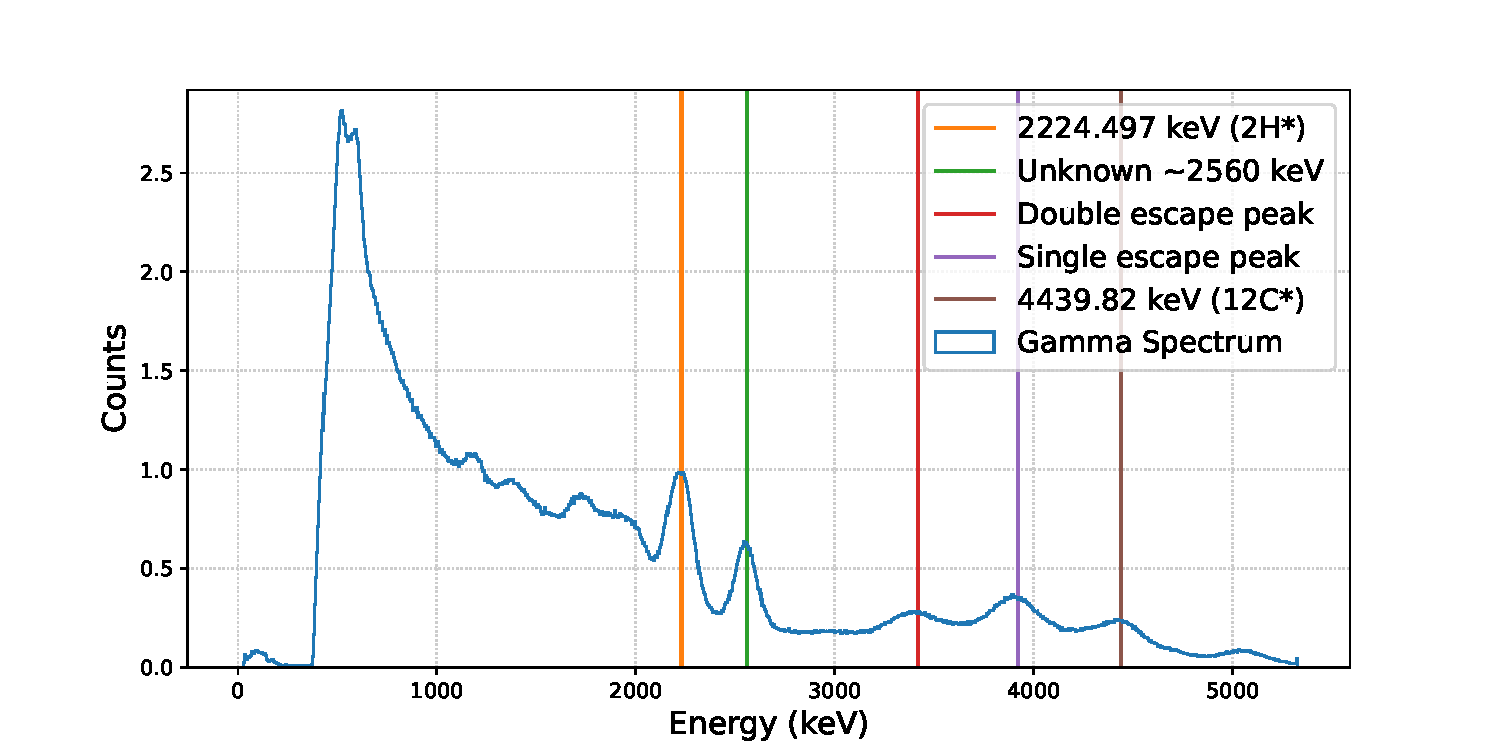
\includegraphics[width=.8\textwidth]{Plots/ambe.pdf}
        \caption{Gamma=ray spectrum for the AmBe source. The expected peaks are identified but the peak at around \SI{2560}{\kilo\electronvolt} remains a mystery. The large continuum at low energies is mostly bremsstrahlung and Compton continuum. The escape peaks for the deuterium and unknown gamma-ray can also be seen although they are obscured by the bremsstrahlung and Compton continua.}
        \label{fig:AmBe_Spectrum}
    \end{center}
\end{figure}

None of the expected peaks intersect each other within the detector's energy resolution, so there is nothing to conclude in that respect. 

\section{Conclusion}\label{sec:Conclusion}
The gamma-ray spectra of the \ce{^{152}Eu} and AmBe radiation sources were found using a NaI scintillation detector and multi-channel analyser. Two different energy needed to be calibrated for in order to best capture the details of each spectrum. The standard \ce{^{22}Na}, \ce{^{60}Co}, and \ce{^{137}Cs} calibration sources were used for this as well as for determining the energy resolution of the NaI detector, which was found to be 6.855\%. 

In each case, the expected energies of the most prominent photopeaks were determined, either by looking them up on NuDat~\cite{nudat} or by determining the theoretical energy by means of a binding energy calculation. These were then compared to the observed photopeaks. In the case of \ce{^{152}Eu}, the energy calibration was found to likely have an incorrect value for the slope of the function. The AmBe calibration appeared to be reasonable but a peak was found in the spectrum at ~\SI{2560}{\kilo\electronvolt} that was not explained by experimental or theoretical expectation. 

\printbibliography

\end{document}